% ===================================================
\chapter{Region-Level Code Replication (RLCR)}
\label{chap:region-level}
% ===================================================

\section{Overview}
Region-Level Code Replication (RLCR) represents the broadest form of software redundancy.
At this level, the entire program image---or a major executable region---is duplicated in full.
Each region contains a complete, self-consistent copy of all code and static data required for execution.
During initialization, a validation routine examines each region to verify its integrity (e.g., via checksum or hash).
Once a valid region is identified, control is transferred to its entry point, and all subsequent execution proceeds entirely within that region.
Because all addresses within a region are internally consistent, no runtime indirection is required after the selection step.

\section{Mechanism}
RLCR operation consists of three stages: replication, validation, and selection.

\paragraph{Replication.}
Redundant regions are produced during the build process, where identical program images are generated and placed at distinct memory addresses.
Each image can be stored in separate non-volatile segments.

\paragraph{Validation.}
At startup, an integrity check is performed for each region.
This routine determines which copy remains intact and therefore safe for execution.

\paragraph{Selection.}
After validation, the system activates the valid region by updating the program counter or vector-table base to the region's start address.
From that point forward, all execution uses fixed absolute addresses within the selected copy.

\begin{figure}[t]
  \centering
  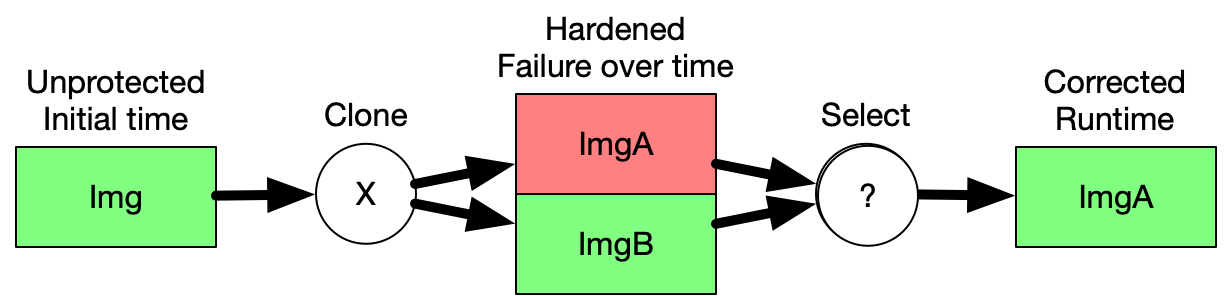
\includegraphics[width=\linewidth]{Chapter-6/figs/dual-image-mechanism.png}
  \caption{Dual-image RLCR mechanism.
           Two identical program regions (ImgA and ImgB) occupy distinct memory ranges.
           On startup, each region is validated; if one fails integrity checks, execution proceeds from the other.
           After a valid region is selected, control remains within that region without further indirection.}
  \label{fig:rlcr-dual}
\end{figure}


\section{Execution Sequence}
Figure~\ref{fig:rlcr-seq} illustrates the loader/selector flow for RLCR.
A minimal loader image performs initialization, invokes a selector when multiple images are present, and then transfers control to the selected program region.
After selection, execution continues entirely within the chosen region.

\begin{figure}[t]
  \centering
  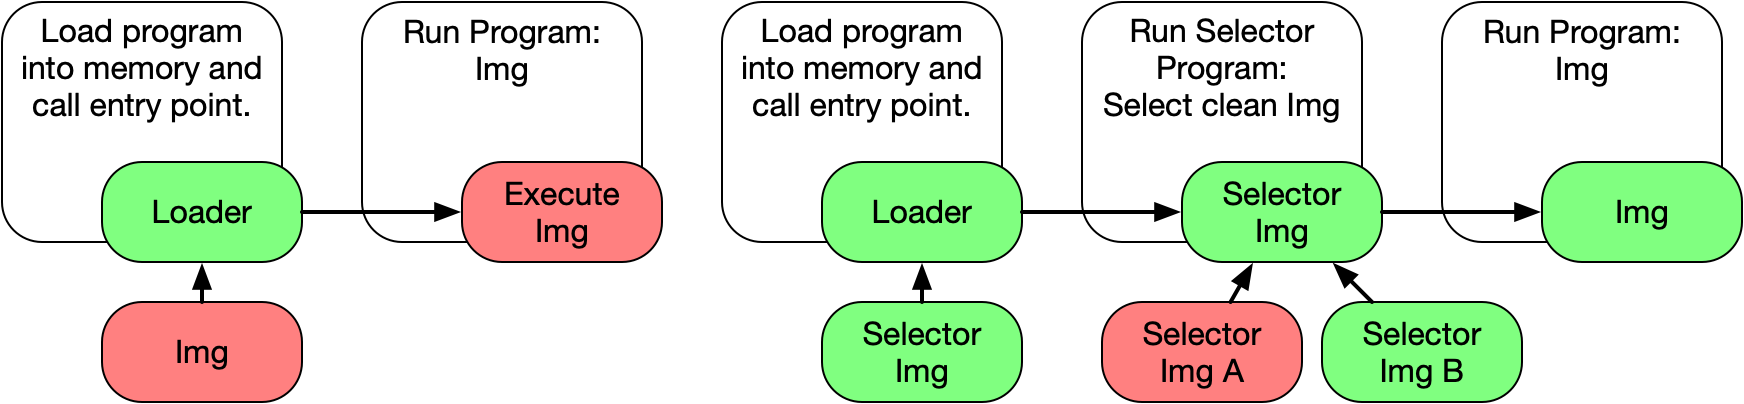
\includegraphics[width=\linewidth]{Chapter-6/figs/rlcr-sequence.png}
  \caption{RLCR execution sequence.
           The loader initializes the system, validates available images (single- or dual-image configurations),
           and transfers control to the first valid region.}
  \label{fig:rlcr-seq}
\end{figure}

\section{Evaluation Setup}
RLCR is evaluated using a dual-image configuration in which two identical program regions share the same total redundancy capacity used in later schemes.
Fault injection introduces persistent errors into non-volatile memory to emulate realistic corruption scenarios.
At startup, the validation routine performs integrity checks and selects the first valid image.
The following measurements are collected:
\begin{itemize}
  \item \textbf{Survivability:} probability that at least one region remains valid after fault injection.
  \item \textbf{Startup latency:} time required for integrity checks and region selection.
  \item \textbf{Memory overhead:} total space occupied by the replicated images.
\end{itemize}
This baseline establishes a reference against which finer-granularity replication methods will be compared in later chapters.

\section{Results}
Experiments confirm that RLCR maintains correct execution whenever at least one region validates successfully.
Since all runtime control flow occurs within the selected image, execution behavior after selection matches that of a non-replicated program.
Validation time scales with region size, and survivability follows the probabilistic model defined earlier as a function of region capacity ($R$) and replication count ($N$).
These results provide the foundation for understanding how finer-granularity approaches refine fault containment while preserving the same total redundancy capacity.

\section{Limit Study (Placeholder)}
\label{sec:rlcr-limit-study}
This section will present the limit study for Region-Level Code Replication once experimental data becomes available.
It will follow the same structure as the \emph{Repair Limit Study}, including:
\begin{itemize}
  \item Experimental configuration and parameters (e.g., number of replicated regions, fault injection rate, validation granularity).
  \item Quantitative results showing survivability and system startup cost as functions of redundancy and fault density.
  \item Comparative discussion of observed saturation points, where additional redundancy yields diminishing returns.
\end{itemize}
At this stage, the section serves as a placeholder for the forthcoming data analysis and figures.

\section{Summary}
RLCR duplicates complete program regions, verifies them at startup, and selects one region for execution.
After selection, control flow is direct and unmodified within the chosen region; no runtime redirection is required.
This chapter establishes the baseline for subsequent techniques---Function-Level and Basic-Block-Level replication---which introduce runtime redirection at progressively finer points in the control flow while keeping overall redundancy storage constant.